\documentclass{beamer}

\usepackage{color}			 % highlight
\usepackage{alltt}			 % highlight

\usepackage{tikz}
\usetikzlibrary{shapes,arrows,calc}
\tikzstyle{block} = [rectangle, draw, text width=5em, text centered]
\tikzstyle{arrow} = [draw, -latex']
\tikzstyle{line} = [draw]

\usepackage{pgfplots}
\pgfplotsset{compat=1.9}

\usepackage{hyperref}
\mode<presentation>

\title{Data Mining \& Differential Privacy}
\author{Mihai Maruseac}

\setbeamertemplate{frametitle continuation}[from second]
%\setbeamertemplate{footline}[frame number]
\setbeamercolor{postit}{fg=black,bg=example text.fg!75!black!10!bg}

\renewcommand\quote[3]{
  \begin{beamercolorbox}[wd=\textwidth,rounded=true,shadow=true]{postit}
    #3
    \vskip5mm
    \hspace*\fill{\small{#1, \textit{#2}}}
  \end{beamercolorbox}
}

\pgfdeclareimage[height=9cm]{netflix}{img/netflix}
\pgfdeclareimage[height=7cm]{hiv}{img/hiv}
\pgfdeclareimage[height=5cm]{graph}{img/graph}
\pgfdeclareimage[height=5cm]{apples}{img/apples}
\pgfdeclareimage[height=4cm]{workflow}{img/workflow}

\pgfdeclareimage[height=3cm]{waterfall}{img/waterfall}
\pgfdeclareimage[height=5cm]{gdp}{img/gdp}

\begin{document}

\maketitle

\begin{frame}{Context}
  \begin{itemize}[<+->]
    \item big data, stream of information
    \item important applications publishing sensitive data about individuals
      \begin{itemize}
        \item medical research
          \begin{itemize}
            \item best treatments
            \item better diagnosis
            \item mapping drugs to phenotypes
          \end{itemize}
        \item public health
          \begin{itemize}
            \item patterns of disease spreading
          \end{itemize}
        \item web search
          \begin{itemize}
            \item better search results
            \item better recommendations
            \item authoritative answers
          \end{itemize}
      \end{itemize}
  \end{itemize}
\end{frame}

\begin{frame}{Context (2)}
  \begin{itemize}
    \item big data, stream of information
  \end{itemize}
  \begin{itemize}[<+->]
    \item important applications publishing sensitive data about individuals
      \begin{itemize}
        \item urban planning
          \begin{itemize}
            \item home, workplace, leisure -- tracked by GPS
            \item travel patterns, experience, cost (time and money)
          \end{itemize}
        \item energy conservation
          \begin{itemize}
            \item patterns of usage
            \item changing the behaviour to better via smart appliances / on
              demand energy sources
          \end{itemize}
        \item networking
          \begin{itemize}
            \item pattern of infrastructure usage
            \item handle exceptional traffic
            \item relationships between people (Facebook, etc.)
            \item census data, society evolution
          \end{itemize}
        \item industrial data
          \begin{itemize}
            \item details about sales, income, customers, costs, etc.
          \end{itemize}
        \item workflows
      \end{itemize}
  \end{itemize}
\end{frame}

\begin{frame}{Context :: Access}
  \color{red}{Access strictly controlled}
  \begin{itemize}[<+->]
    \item only inside company/agency which collected the data
    \item only after signing a special contract (taxi, click streams)
    \item only in coarse-grained summaries (health)
    \item only after a long wait (census)
    \item only with 3-letters-organisations approval
  \end{itemize}
\end{frame}

\begin{frame}{Context :: Issues}
  \begin{itemize}
    \item access to data strictly controlled
    \item data released with privacy issues (AOL click stream)
  \end{itemize}
  \begin{beamercolorbox}[wd=\textwidth,rounded=true,shadow=true]{postit}
    Society would benefit if we could publish useful data without
    worrying about privacy and access issues.
  \end{beamercolorbox}
\end{frame}

\begin{frame}{Privacy}
  \begin{itemize}[<+->]
    \item na\"ive solution: remove sensitive columns
    \item cross table references
    \item \color{red}{87\% Americans uniquely identified by \texttt{zip,
      gender, birthdate}}
    \item 2002, medical records of Governor of MA
  \end{itemize}
\end{frame}

\begin{frame}{Privacy (2)}
  \begin{itemize}[<+->]
    \item query logs: useful for CS researchers, system admins, etc.
    \item find all AOL logs of user 4417749
    \item multiple queries for services in Lilburn, GA
    \item population 11,000
    \item some queries for Jarret Arnold
    \item 14 people with this name in Lilburn
    \item contact each of them / social engineering
    \item AOL user 4417749 = Thelma Arnold
  \end{itemize}
\end{frame}

\begin{frame}{Privacy (3)}
  \begin{itemize}[<+->]
    \item Netflix prize (2009, 1M\$)
    \item training data: 100M ratings from 18K movies of 500K customers
    \item 10\% of data slightly disturbed
    \item use blogs, FB posts, twitters post, IMDB profiles to identify users
      \begin{itemize}
        \item 8 ratings, dates within 2 weeks -- 99\% of raters
        \item 2 ratings, dates within 3 days -- 68\% of raters
        \item all raters of top 100 movies
        \item IMDB comments -- Netflix reidentification
      \end{itemize}
  \end{itemize}
\end{frame}

\begin{frame}{}
  \center{\pgfuseimage{netflix}}
\end{frame}

\begin{frame}{}
  \begin{beamercolorbox}[wd=\textwidth,rounded=true,shadow=true]{postit}
    One customer $\ldots$ sued Netflix, saying she thought her rental
    history could reveal that she was a lesbian before she was ready to tell
    everyone.
  \end{beamercolorbox}
\end{frame}

\begin{frame}{}
  \center{\pgfuseimage{hiv}}
\end{frame}

\begin{frame}{}
  \center{\pgfuseimage{graph}}
\end{frame}

\begin{frame}{Important note}
  \begin{beamercolorbox}[wd=\textwidth,rounded=true,shadow=true]{postit}
    Just because data looks hard to re-identify, doesn't mean it \textit{is}.
  \end{beamercolorbox}
\end{frame}

\begin{frame}{Solution}
  \begin{beamercolorbox}[wd=\textwidth,rounded=true,shadow=true]{postit}
    Publish a distorted version of the data.
  \end{beamercolorbox}
  \pause
  \begin{description}
    \item[privacy] privacy ``adequately'' protected
    \item[utility] information is useful for its intended purpose
  \end{description}
  \pause
  \begin{beamercolorbox}[wd=\textwidth,rounded=true,shadow=true]{postit}
    privacy $\nearrow$, utility $\searrow$
  \end{beamercolorbox}
\end{frame}

\begin{frame}{Privacy protection needs}
  \begin{itemize}
    \item membership disclosure: is $X$ in $Xs$?
    \item sensitive attribute disclosure: has $X$ $a$?
    \item identity disclosure: does $i$ belong to $X$? are $x$ and $y$ the
      same?
  \end{itemize}
\end{frame}

\begin{frame}{$k$-anonymity}
  \begin{beamercolorbox}[wd=\textwidth,rounded=true,shadow=true]{postit}
    Your quasi-identifiers are indistinguishable from at least other $k$
    people's.
  \end{beamercolorbox}
  \pause
  \begin{itemize}
    \item easy to understand
    \item easy to attack
      \begin{itemize}
        \item doesn't say anything about operations done on data
        \item join on other columns
        \item no protection against background knowledge
        \item updates (age) destroy protection
      \end{itemize}
  \end{itemize}
\end{frame}

\begin{frame}{Other approaches}
  \begin{description}
    \item[$l$-diversity]: each group must have at least $l$ distinct values
    \item[probabilistic $l$-diversity]: frequency of the most frequent value
      in a class is bounded by $1/l$
    \item[entropy $l$-diversity]: entropy of distribution of values inside a
      class is at least $\log(l)$
    \item[recursive $(c, l)$-diversity]
    \item[$\ldots$] ($>$ 100 related approaches)
  \end{description}
  \pause
  \begin{itemize}
    \item hard to achieve
    \item underkill/overkill
  \end{itemize}
\end{frame}

\begin{frame}{Fatal flaws of privacy by syntactic transformation of data}
  \begin{itemize}
    \item insecure against attackers with too much background info
    \item no composition
    \item no meaningful definitions for privacy and utility
    \item no mathematic guarantees of protection.
  \end{itemize}
  \pause
  \begin{beamercolorbox}[wd=\textwidth,rounded=true,shadow=true]{postit}
    Privacy is \textbf{not} a property of the data.
  \end{beamercolorbox}
  \begin{itemize}
    \item privacy depends on the analysis done on the data
    \item identity transformation
  \end{itemize}
\end{frame}

\begin{frame}{Differential Privacy}
  \begin{beamercolorbox}[wd=\textwidth,rounded=true,shadow=true]{postit}
    An analysis result should not change much when adding/removing a single
    tuple.
  \end{beamercolorbox}
  \pause
  \begin{beamercolorbox}[wd=\textwidth,rounded=true,shadow=true]{postit}
    Each user should not be worse off by having its record in the database.
  \end{beamercolorbox}
  \pause
  \begin{equation*}
    e^{-\epsilon} \le \frac{Pr(\mathcal{A}(Q, D_1) = R)}{Pr(\mathcal{A}(Q, D_2) = R)} \le e^{\epsilon}
  \end{equation*}
\end{frame}

\begin{frame}{Differential Privacy (2)}
  \begin{beamercolorbox}[wd=\textwidth,rounded=true,shadow=true]{postit}
    Add noise to analysis result.
  \end{beamercolorbox}
  \pause
  \begin{itemize}
    \item sensibility of result (query)
    \item the more sensible the result, the more noise needs to be added
    \item sensibility is \textit{worst-case} measure
    \item sensibility is independent of data in database
    \item sensibility of \textit{how many people have this disease?} is 1
    \item sensibility of \textit{what's the average salary of employees} is
      very high (sum, max, min, $\ldots$)
  \end{itemize}
\end{frame}

\begin{frame}{Differential Privacy (3)}
  \begin{beamercolorbox}[wd=\textwidth,rounded=true,shadow=true]{postit}
    How to define sensibility?
  \end{beamercolorbox}
  \pause
  \begin{itemize}
    \item what can we publish?
      \pause
      \begin{description}
        \item[YES] average height
        \item[NO] individual height
      \end{description}
      \pause
    \item add 1m to height of one person: what changes?
  \end{itemize}
  \pause
  \begin{equation*}
    \Delta(f) = \max_{D_1, D_2} \| f(D_1) - f(D_2) \|
  \end{equation*}
\end{frame}

\begin{frame}{Differential Privacy (4)}
  \begin{beamercolorbox}[wd=\textwidth,rounded=true,shadow=true]{postit}
    Laplace mechanism
  \end{beamercolorbox}
  \pause
  \begin{eqnarray*}
    \tilde x &=& x + Lap(\lambda)\\
    Lap(\lambda) &=& \frac{1}{2\lambda}\exp(-\frac{|x|}{\lambda})\\
    \lambda &=& \frac{\Delta(f)}{\epsilon}
  \end{eqnarray*}
  \begin{center}
    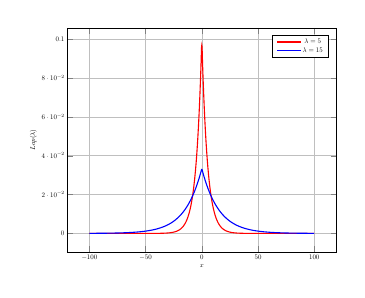
\begin{tikzpicture}[auto, scale=0.5, every node/.style={scale=0.5}]
    \begin{axis}[domain=-100:100,
        samples=500,
        grid=major,smooth,
        xlabel=$x$,
        ylabel=$Lap(\lambda)$,
        legend pos=north east]
    \addplot [color=red,thick] {(1/(2*5))*exp(-abs(x)/5)};
    \addplot [color=blue,thick] {(1/(2*15))*exp(-abs(x)/15)};
    \legend {$\lambda = 5$, $\lambda = 15$};
    \end{axis}
    \end{tikzpicture}
  \end{center}
\end{frame}

\begin{frame}{Laplace mechanism :: example}
  \begin{itemize}[<+->]
    \item How many users viewed more than 10 movies?
    \item sensibility: $\Delta(f) = 1$
    \item actual result: $x = 42$
    \item $\epsilon = 0.1$, $\lambda = 10$
    \item (possible) output: $\tilde x = 37$ (noise -5)
  \end{itemize}
\end{frame}

\begin{frame}{Differential Privacy (5)}
  \begin{beamercolorbox}[wd=\textwidth,rounded=true,shadow=true]{postit}
    Exponential mechanism
  \end{beamercolorbox}
  \pause
  \begin{itemize}
    \item Laplace mechanism works for numerical data
    \item Exponential mechanism works for categorical data
    \item each item has a quality function $q(x)$
    \item randomly output item with probability $\sim \exp(\frac{q(x)}{\lambda})$
    \item $\lambda = \frac{2\Delta(q)}{\epsilon}$
  \end{itemize}
\end{frame}

\begin{frame}{Exponential mechanism :: example}
  \begin{center}
    \pgfuseimage{apples}
  \end{center}
\end{frame}

\begin{frame}{Differential Privacy (6)}
  \begin{beamercolorbox}[wd=\textwidth,rounded=true,shadow=true]{postit}
    Composability
  \end{beamercolorbox}
  \pause
  \begin{description}
    \item[sequential composition] $\epsilon_t = \epsilon_1 + \epsilon_2 + \ldots + \epsilon_k$
    \item[parallel composition] $\epsilon_t = \max\left\{\epsilon_1,\epsilon_2,\ldots,\epsilon_k\right\}$
  \end{description}
\end{frame}

\begin{frame}{Differential Privacy (7)}
  \begin{beamercolorbox}[wd=\textwidth,rounded=true,shadow=true]{postit}
    How to use the mechanisms?
  \end{beamercolorbox}
  \pause
  \begin{itemize}
    \item using them directly gives not so good results
    \item composability properties help
    \item we can generate synthetic data and apply all algorithms on that
    \item we can interleave dp mechanisms with the original data-mining
      algorithm
    \item optimization problems
  \end{itemize}
\end{frame}

\begin{frame}{Workflow}
  \begin{beamercolorbox}[wd=\textwidth,rounded=true,shadow=true]{postit}
    Paths in organisation.
  \end{beamercolorbox}
  \begin{center}
    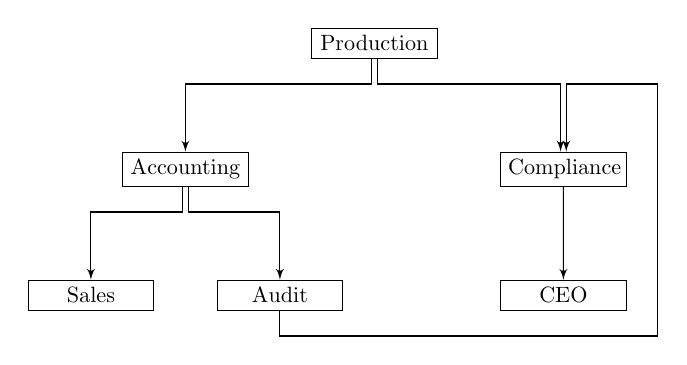
\begin{tikzpicture}[node distance = 3cm, auto, scale=0.8, every node/.style={scale=0.8}]
      \pgfmathsetmacro{\dx}{1.5}
      \pgfmathsetmacro{\dy}{-2}
      \pgfmathsetmacro{\sepx}{0.03}
      \pgfmathsetmacro{\sepy}{0.2}
      \node [block] at (0, 0) (d1) {Production};
      \node [block] at (-2 * \dx,     \dy) (d2) {Accounting};
      \node [block] at (-3 * \dx, 2 * \dy) (d3) {Sales};
      \node [block] at (-1 * \dx, 2 * \dy) (d4) {Audit};
      \node [block] at ( 2 * \dx,     \dy) (d5) {Compliance};
      \node [block] at ( 2 * \dx, 2 * \dy) (d6) {CEO};
      \coordinate (d5p1) at ($(d5.north) + (-\sepx * \dx, 0)$);
      \coordinate (d5p2) at ($(d5.north) + ( \sepx * \dx, 0)$);
      \path [arrow] (d1.south) -- +(- \sepx * \dx, 0) -- +(- \sepx * \dx, \sepy * \dy) -| (d2);
      \path [arrow] (d1.south) -- +(  \sepx * \dx, 0) -- +(  \sepx * \dx, \sepy * \dy) -| (d5p1);
      \path [arrow] (d2.south) -- +(- \sepx * \dx, 0) -- +(- \sepx * \dx, \sepy * \dy) -| (d3);
      \path [arrow] (d2.south) -- +(  \sepx * \dx, 0) -- +(  \sepx * \dx, \sepy * \dy) -| (d4);
      \path [arrow] (d5) -- (d6);
      \path [arrow] (d4.south) -- +(0, \sepy * \dy) -- +(4 * \dx, \sepy * \dy) -- +(4 * \dx, -2 * \dy + \sepy * \dy) -| (d5p2);
    \end{tikzpicture}
  \end{center}
\end{frame}

\begin{frame}{Workflow (2)}
  \begin{beamercolorbox}[wd=\textwidth,rounded=true,shadow=true]{postit}
    How many docs go through $i \rightarrow j \rightarrow k$
  \end{beamercolorbox}
  \begin{center}
    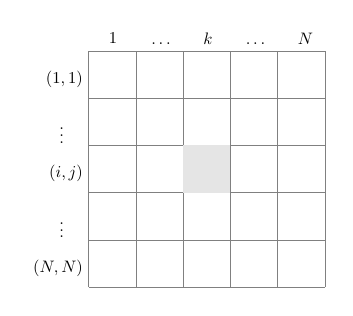
\begin{tikzpicture}[auto, scale=0.6, every node/.style={scale=0.6}]
      \draw[style=help lines] (0,0) grid (5, 5);

      \fill[gray!20] (2,2) -- (2,3) -- (3,3) -- (3,2) -- cycle;

      \node at (0.3, 5.5) [anchor=north west] {$1$};
      \node at (1.2, 5.3) [anchor=north west] {$\ldots$};
      \node at (2.3, 5.5) [anchor=north west] {$k$};
      \node at (3.2, 5.3) [anchor=north west] {$\ldots$};
      \node at (4.3, 5.5) [anchor=north west] {$N$};
      \node at (0, 4.7) [anchor=north east] {$(1, 1)$};
      \node at (-0.4, 3.7) [anchor=north east] {$\vdots$};
      \node at (0, 2.7) [anchor=north east] {$(i, j)$};
      \node at (-0.4, 1.7) [anchor=north east] {$\vdots$};
      \node at (0, 0.7) [anchor=north east] {$(N, N)$};
    \end{tikzpicture}
  \end{center}
\end{frame}

\begin{frame}{Workflow (3)}
  \begin{beamercolorbox}[wd=\textwidth,rounded=true,shadow=true]{postit}
    How many triangle paths ($i \rightarrow j \rightarrow i$)
  \end{beamercolorbox}
  \begin{center}
    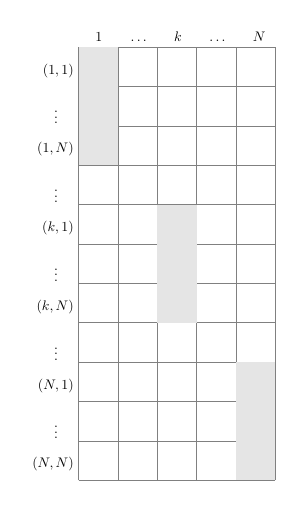
\begin{tikzpicture}[auto, scale=0.5, every node/.style={scale=0.5}]
      \draw[style=help lines] (0,0) grid (5, 11);

      \fill[gray!20] (4,0) -- (4,3) -- (5,3) -- (5,0) -- cycle;
      \fill[gray!20] (2,4) -- (2,7) -- (3,7) -- (3,4) -- cycle;
      \fill[gray!20] (0,8) -- (0,11) -- (1,11) -- (1,8) -- cycle;

      \node at (0.3, 11.5) [anchor=north west] {$1$};
      \node at (1.2, 11.3) [anchor=north west] {$\ldots$};
      \node at (2.3, 11.5) [anchor=north west] {$k$};
      \node at (3.2, 11.3) [anchor=north west] {$\ldots$};
      \node at (4.3, 11.5) [anchor=north west] {$N$};
      \node at (0, 10.7) [anchor=north east] {$(1, 1)$};
      \node at (-0.4, 9.7) [anchor=north east] {$\vdots$};
      \node at (0, 8.7) [anchor=north east] {$(1, N)$};
      \node at (-0.4, 7.7) [anchor=north east] {$\vdots$};
      \node at (0, 6.7) [anchor=north east] {$(k, 1)$};
      \node at (-0.4, 5.7) [anchor=north east] {$\vdots$};
      \node at (0, 4.7) [anchor=north east] {$(k, N)$};
      \node at (-0.4, 3.7) [anchor=north east] {$\vdots$};
      \node at (0, 2.7) [anchor=north east] {$(N, 1)$};
      \node at (-0.4, 1.7) [anchor=north east] {$\vdots$};
      \node at (0, 0.7) [anchor=north east] {$(N, N)$};
    \end{tikzpicture}
  \end{center}
\end{frame}

\begin{frame}{Workflow (4)}
  \begin{beamercolorbox}[wd=\textwidth,rounded=true,shadow=true]{postit}
    How many returned docs ($i \rightarrow \ldots j \rightarrow \ldots i$)
  \end{beamercolorbox}
  \begin{center}
    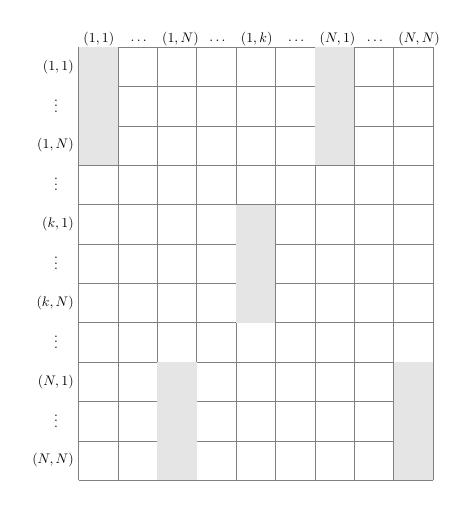
\begin{tikzpicture}[auto, scale=0.5, every node/.style={scale=0.5}]
      \draw[style=help lines] (0,0) grid (9, 11);

      \fill[gray!20] (0,8) -- (0,11) -- (1,11) -- (1,8) -- cycle;
      \fill[gray!20] (6,8) -- (6,11) -- (7,11) -- (7,8) -- cycle;
      \fill[gray!20] (4,4) -- (4,7) -- (5,7) -- (5,4) -- cycle;
      \fill[gray!20] (2,0) -- (2,3) -- (3,3) -- (3,0) -- cycle;
      \fill[gray!20] (8,0) -- (8,3) -- (9,3) -- (9,0) -- cycle;

      \node at (0.0, 11.5) [anchor=north west] {$(1, 1)$};
      \node at (1.2, 11.3) [anchor=north west] {$\ldots$};
      \node at (2.0, 11.5) [anchor=north west] {$(1, N)$};
      \node at (3.2, 11.3) [anchor=north west] {$\ldots$};
      \node at (4.0, 11.5) [anchor=north west] {$(1, k)$};
      \node at (5.2, 11.3) [anchor=north west] {$\ldots$};
      \node at (6.0, 11.5) [anchor=north west] {$(N, 1)$};
      \node at (7.2, 11.3) [anchor=north west] {$\ldots$};
      \node at (8.0, 11.5) [anchor=north west]{$(N, N)$};
      \node at (0, 10.8) [anchor=north east] {$(1, 1)$};
      \node at (-0.4, 10.0) [anchor=north east] {$\vdots$};
      \node at (0, 8.8) [anchor=north east] {$(1, N)$};
      \node at (-0.4, 8.0) [anchor=north east] {$\vdots$};
      \node at (0, 6.8) [anchor=north east] {$(k, 1)$};
      \node at (-0.4, 6.0) [anchor=north east] {$\vdots$};
      \node at (0, 4.8) [anchor=north east] {$(k, N)$};
      \node at (-0.4, 4.0) [anchor=north east] {$\vdots$};
      \node at (0, 2.8) [anchor=north east] {$(N, 1)$};
      \node at (-0.4, 2.0) [anchor=north east] {$\vdots$};
      \node at (0, 0.8) [anchor=north east] {$(N, N)$};
    \end{tikzpicture}
  \end{center}
\end{frame}

\begin{frame}{Workflow (5)}
  \begin{itemize}
    \item n-gram model for higher dimensionality
    \item integrity constraints
  \end{itemize}
  \begin{center}
    \pgfuseimage{workflow}
  \end{center}
\end{frame}

\begin{frame}{Differential Privacy (8)}
  \begin{beamercolorbox}[wd=\textwidth,rounded=true,shadow=true]{postit}
    Limitations
  \end{beamercolorbox}
  \begin{itemize}
    \item results are worse for higly-corellated data
    \item no extensions for complex models
    \item how to properly set $\epsilon$
    \item expensive computations
    \item error bounds
    \item no direct relationship between utility and privacy
    \item inconsistencies
  \end{itemize}
\end{frame}
\end{document}
